\documentclass{ctexart}

\usepackage{cite}
\usepackage{amsmath}
\usepackage{algorithm}
\usepackage{algorithmic}
\usepackage{graphicx}
\usepackage{amsthm}
\usepackage{amssymb}

\title{SVD和随机投影两种降维方法在K-means中的应用}
\author{李纯羽 \and 樊金昊}
\begin{document}
    \maketitle

    \begin{abstract}
        降维的方法包括特征选择和特征提取两种,本文使用SVD作为特征选择方法和随机投影作为特征提取方法,对ORL人脸数据集以及其他数据集(改)进行降维,并使用k-means对降维之后的结果进行聚类。我们比较了两种方法,并分别进行了一些优化。
    \end{abstract}
    \tableofcontents
    \newpage

    \section{基于随机投影的降维方法}

    \subsection{背景和引入}
        随机投影属于特征提取方法的一种,所依据的原理是JL 引理,即经过线性变换f之后原点集中两个点的距离仍然在一定误差范围内保持,这样的性质适合在k-means中使用。

        K-means的目标函数用矩阵表示为
        \begin{equation*}
            X_{opt} = \mathop{\arg\min}_{X \in \chi} \| A - XX^{\top}A \|_{F}^2 \label{opt}
        \end{equation*}

        其中X表示聚类的结果,当且仅当第i个点属于第j类的时候$X_{ij}$非零,并且$X_{ij}= 1/\sqrt{z_{j}}$, 其中$z_{j}$表示在对应类中的点的数量,这样就保证了后面一项表示各点所属的类类中心的位置。

        在这个实验中我们使用Lloyd算法实现k-means聚类,虽然这个算法没有最差保证,但是通过初始点的选择保证聚类的效果不会很差。

    \subsection{算法描述和时间复杂度分析}
    \subsubsection{算法描述}
    \renewcommand{\algorithmicrequire}{ \textbf{Input:}} %Use Input in the format of Algorithm
    \renewcommand{\algorithmicensure}{ \textbf{Output:}} %UseOutput in the format of Algorithm
    \begin{algorithm}[htb]
    \caption{k-means 聚类使用的随机投影算法}
    \label{RP}
        \begin{algorithmic}[1] %这个1 表示每一行都显示数字
        \REQUIRE ~~\\ %算法的输入参数:Input
            矩阵 $ A \in R^{n \times d}$, 类的数目k, 误差因子 $\varepsilon \in (0, 1/3)$, $\gamma$近似的k-means算法. \\
        \ENSURE ~~\\ %算法的输出:Output
            矩阵 $ X_{\tilde{\gamma}} $ 表示聚类结果

        \STATE 设置目标维度 $ t = \Omega(k/\varepsilon^2)$, 对足够大的常数c, $t = t_{0} \ge ck/\varepsilon^2 $;
        \label{ step 1 }%对此行的标记,方便在文中引用算法的某个步骤
        \STATE 产生随机矩阵 $ R \in R^{d \times t} $,对于所有$ i \in [d], j \in [t]$
        \begin{equation*}
        R_{ij} = \begin{cases} +1/\sqrt{t},& \mbox{w.p. 1/2,} \\ -1/\sqrt{t}, & \mbox{w.p. 1/2.}\end{cases}
        \end{equation*}
        \label{step 2}
        \STATE 计算矩阵$\tilde{A} = AR$.
        \label{step 3}
        \STATE 在矩阵$ \tilde{A}$上运行$\gamma$近似的k-means算法得到$X_{\tilde{\gamma}}$;返回矩阵$ X_{\tilde{\gamma}}$
        \label{step 4}
        \end{algorithmic}
    \end{algorithm}

    \subsubsection{时间复杂度分析}
    Lloyd算法一个循环的时间复杂度从$O(knd)$降到了$O(nk^2/\varepsilon^2)$.
    使用$\gamma = 1 + \varepsilon$近似的k-means算法,对于$\forall \varepsilon \in (0, 1/3)$,时间复杂度为$O(nd\lceil\varepsilon^{-2}k/log(d)\rceil + 2^{(k/\varepsilon)^{O(1)}}kn/\varepsilon^2)$.

    \subsubsection{算法的近似比}
    假设上述算法使用$\gamma$近似的k-means算法,则有
    \begin{equation*}
        \| A - X_{\tilde{\gamma}}X_{\tilde{\gamma}}^{\top}A \|_{F}^2 \le (1+(1+\varepsilon)\gamma) \| A - X_{opt}X_{opt}^{\top}A \|_{F}^2
    \end{equation*}

    \subsection{算法近似比的数学证明}
    下面简单的证明上面关于近似比的结论
    \begin{proof}
    $  A = A_{k} + A_{\rho - k} $\\
    其中, $ \rho $ 代表A的秩, $A_{k} = U_{k}\sum_{k}V_{k}, U_{k},V_{k},\sum_{k}$分别是由前k个左右奇异向量和奇异值组成的矩阵.由正交性
    \begin{align*}
    &\| A - X_{\tilde{\gamma}}X_{\tilde{\gamma}}^{\top}A \|_{F}^2 =
     \| (I - X_{\tilde{\gamma}}X_{\tilde{\gamma}}^{\top})A_{k} \|_{F}^2
    + \| (I - X_{\tilde{\gamma}}X_{\tilde{\gamma}}^{\top}) A_{k} \|_{F}^2\\
    &\because
    (I - X_{\tilde{\gamma}}X_{\tilde{\gamma}}^{\top}) \text { 为投影矩阵 }\\
    & \therefore
    \|(I - X_{\tilde{\gamma}}X_{\tilde{\gamma}}^{\top})A_{\rho -k}\|_{F}^2
        \le \|A_{\rho - k}\|_{F}^2 = \|A - A_{k} \|_{F}^2 	
        \le \|A - X_{opt}X_{opt}^{\top}A\|_{F}^2
    \end{align*}

    R为算法产生的随机投影矩阵,
    $E = A_{k} - (AR)(V_{k}^{\top}R)^{\dagger}V_{k}^{\top}$,并且可以证明$\left | \left |E\right | \right | _{F} \le 4\varepsilon\left | \left |A - A_{k}\right | \right | _{F}$,则
    \begin{align*}
    &\|(I - X_{\tilde{\gamma}}X_{\tilde{\gamma}}^{\top})A_{k}\|_{F}\\
    &    \le \|(I - X_{\tilde{\gamma}}X_{\tilde{\gamma}}^{\top})AR(V_{k}^{\top}R)^{\dagger}V_{k}^{\top}\|_{F} + \|E\|_{F}\\
    & \le \|(I - X_{\tilde{\gamma}}X_{\tilde{\gamma}}^{\top})AR\|_{F}\|(V_{k}^{\top}R)^{\dagger}V_{k}^{\top}\|_{2} + \|E\|_{F}\\
    &    \le \|(I - X_{\tilde{\gamma}}X_{\tilde{\gamma}}^{\top})AR\|_{F}\|(V_{k}^{\top}R)^{\dagger}\|_{2} + \|E\|_{F}\\
    &    \because \|(I - X_{\tilde{\gamma}}X_{\tilde{\gamma}}^{\top})AR\|_{F}^2 \le \gamma\mathop{\min}_{X \in \chi}
    \|(I - XX^{\top})AR\|_{F}^2 \le \gamma \|(I - X_{opt}X_{opt}^{\top})AR\|_{F}^2\\
    & \therefore  \|(I - X_{\tilde{\gamma}}X_{\tilde{\gamma}}^{\top})AR\|_{F}\|(V_{k}^{\top}R)^{\dagger}\|_{2} + \|E\|_{F}\\
    &\le \sqrt{\gamma}\|(I - X_{opt}X_{opt}^{\top})AR\|_{F}\|(V_{k}^{\top}R)^{\dagger}\|_{2} + \|E\|_{F}\\
    &\le \sqrt{\gamma}\|(I - X_{opt}X_{opt}^{\top})A\|_{F}\sqrt{1+\varepsilon}\|(V_{k}^{\top}R)^{\dagger}\|_{2} + \|E\|_{F}\\
    &\because \forall i \in [k] |1 - \sigma_{i}(V_{k}^{\top}R)| \le \varepsilon \text{其中} \sigma_{i} \text{表示A的第i个非负奇异值} \\
    &\therefore \|(V_{k}^{\top}R)^{\dagger}\|_{2} \le \frac{1}{1-\varepsilon}\\
    &\therefore \sqrt{\gamma}\|(I - X_{opt}X_{opt}^{\top})A\|_{F}\sqrt{1+\varepsilon}\|(V_{k}^{\top}R)^{\dagger}\|_{2} + \|E\|_{F}\\
    &\le \sqrt{\gamma} \times \frac{\sqrt{1+\varepsilon}}{1-\varepsilon}\|(I - X_{opt}X_{opt}^{\top})A\|_{F}
    + 4\varepsilon \|(I - X_{opt}X_{opt}^{\top})A\|_{F}\\
    &\le \sqrt{\gamma} (1+6.5\varepsilon)\|(I - X_{opt}X_{opt}^{\top})A\|_{F}
    \end{align*}
    \end{proof}

    \subsection{实验复现}
    实验使用ORL人脸数据集,这个数据集包含40类,每一类包含10张人脸图片,因为刚开始没有找到分辨率64*64的数据,使用的是分辨率112 *92 的数据集。由于数据按照类顺序排列,使用Lloyd算法时取每一类的第一张图片作为初始类中心。\\

    选取三个评价指标,分别是
    \begin{itemize}
    \item 归一化的目标函数,表示k-means收敛的情况
    \item 分类的准确率,使用正确分类的图片数除以总数
    \item 从算法第一步开始到结束总的执行时间
    \end{itemize}
    初始维度是10304维,将目标维度t从5增长到300,计算三个评价指标的结果如\ref{1},\ref{2},\ref{3} \\

        \begin{figure}[h]
        \centering
        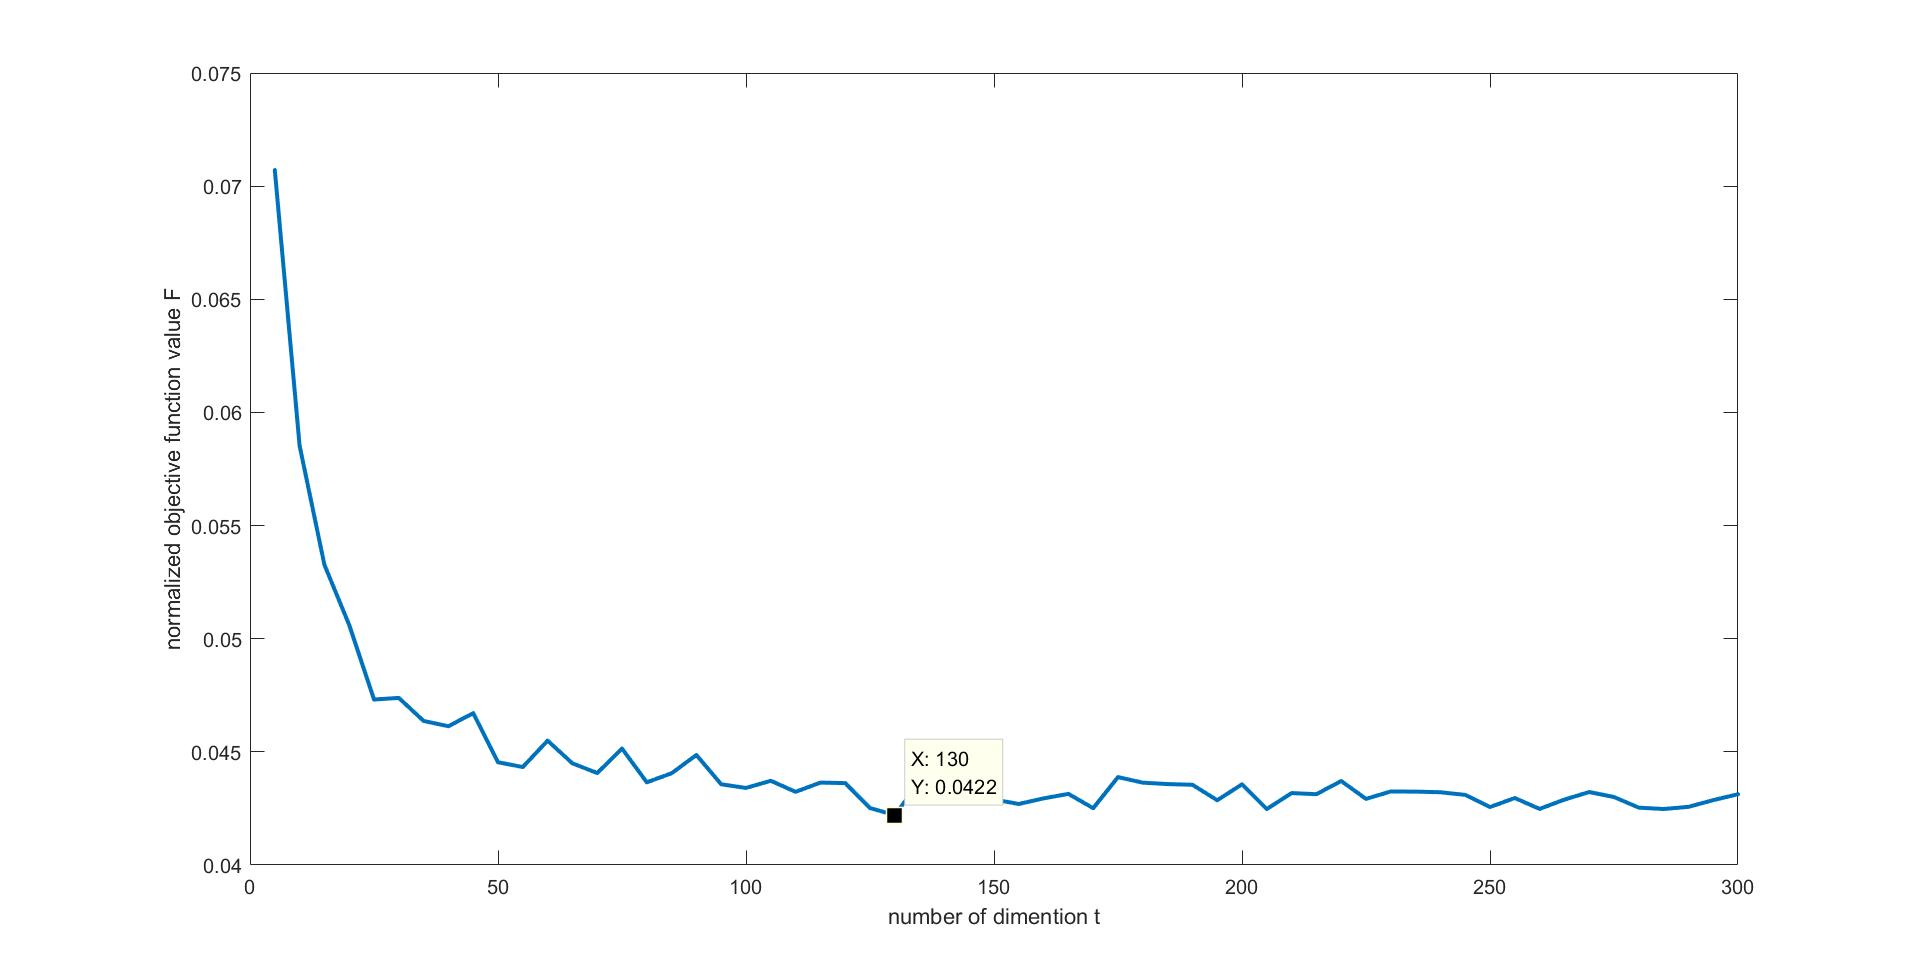
\includegraphics[width=0.50\textwidth]{norm_F.jpg}
        \caption{归一化的目标函数}
        \label{1}
        \end{figure}

        \begin{figure}[h]
        \centering
        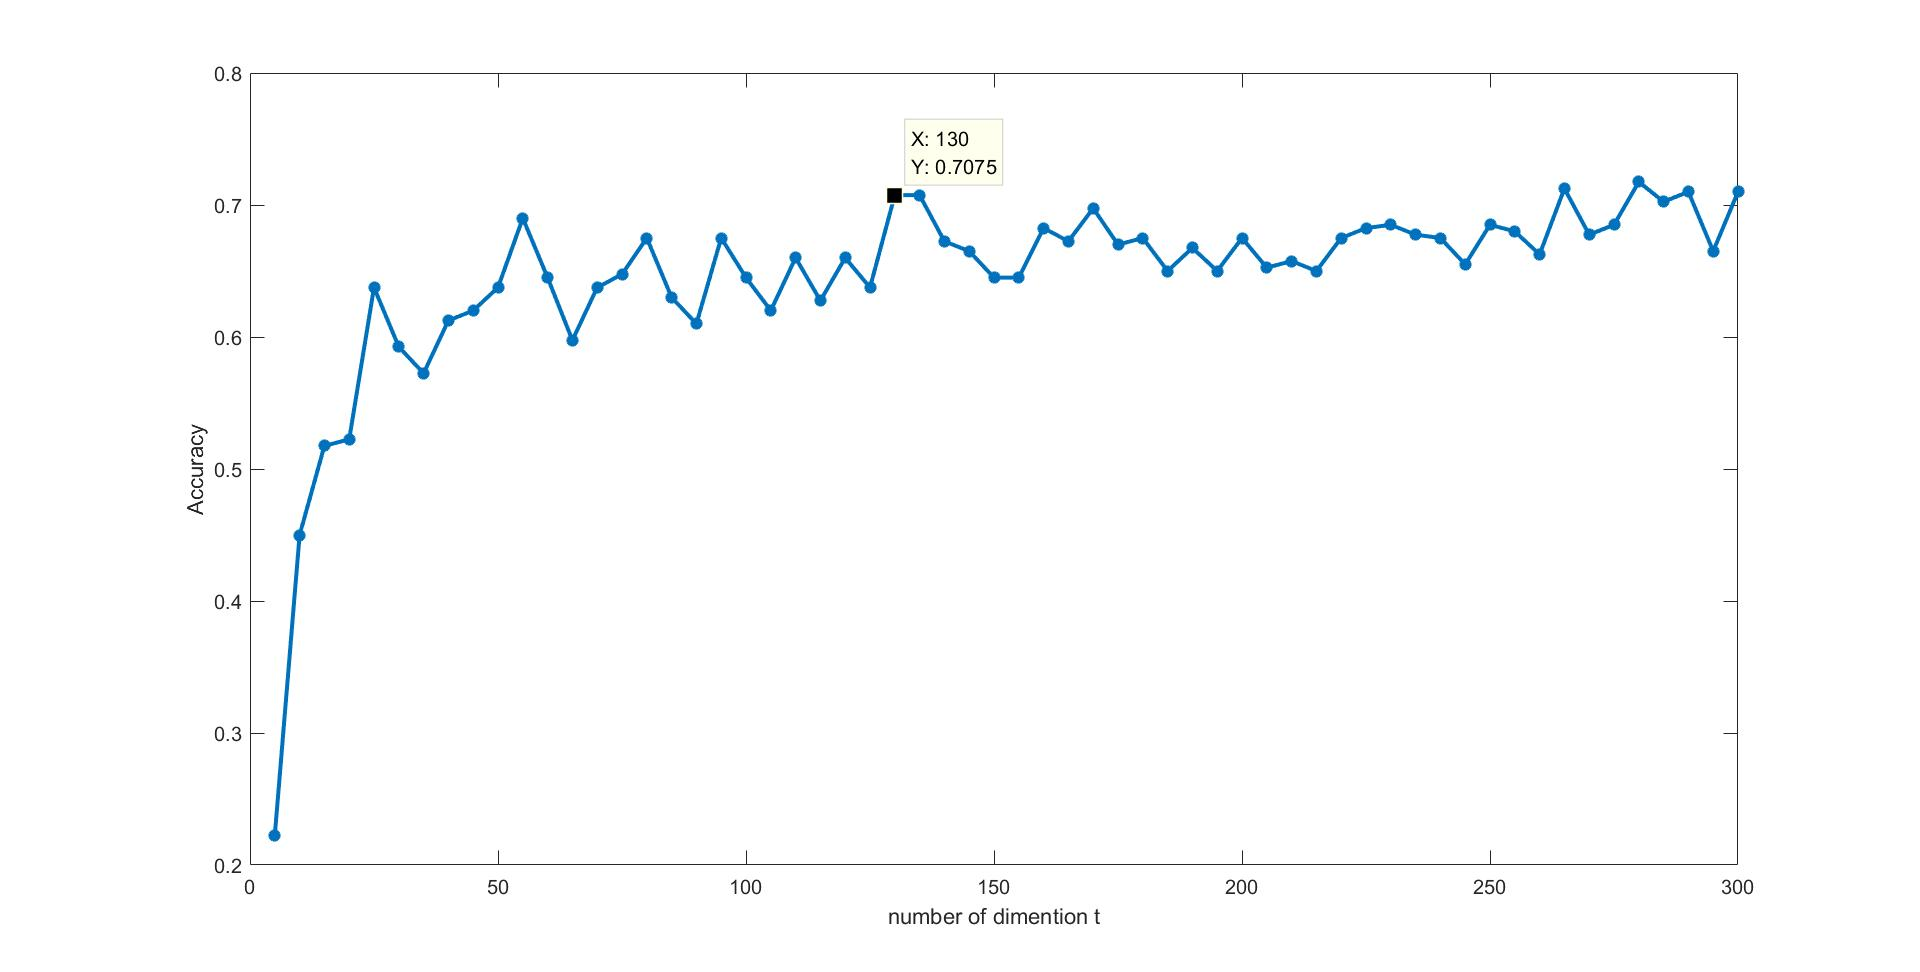
\includegraphics[width=0.50\textwidth]{acc.jpg}
        \caption{分类的准确率}
        \label{2}
        \end{figure}

        \begin{figure}[h]
        \centering
        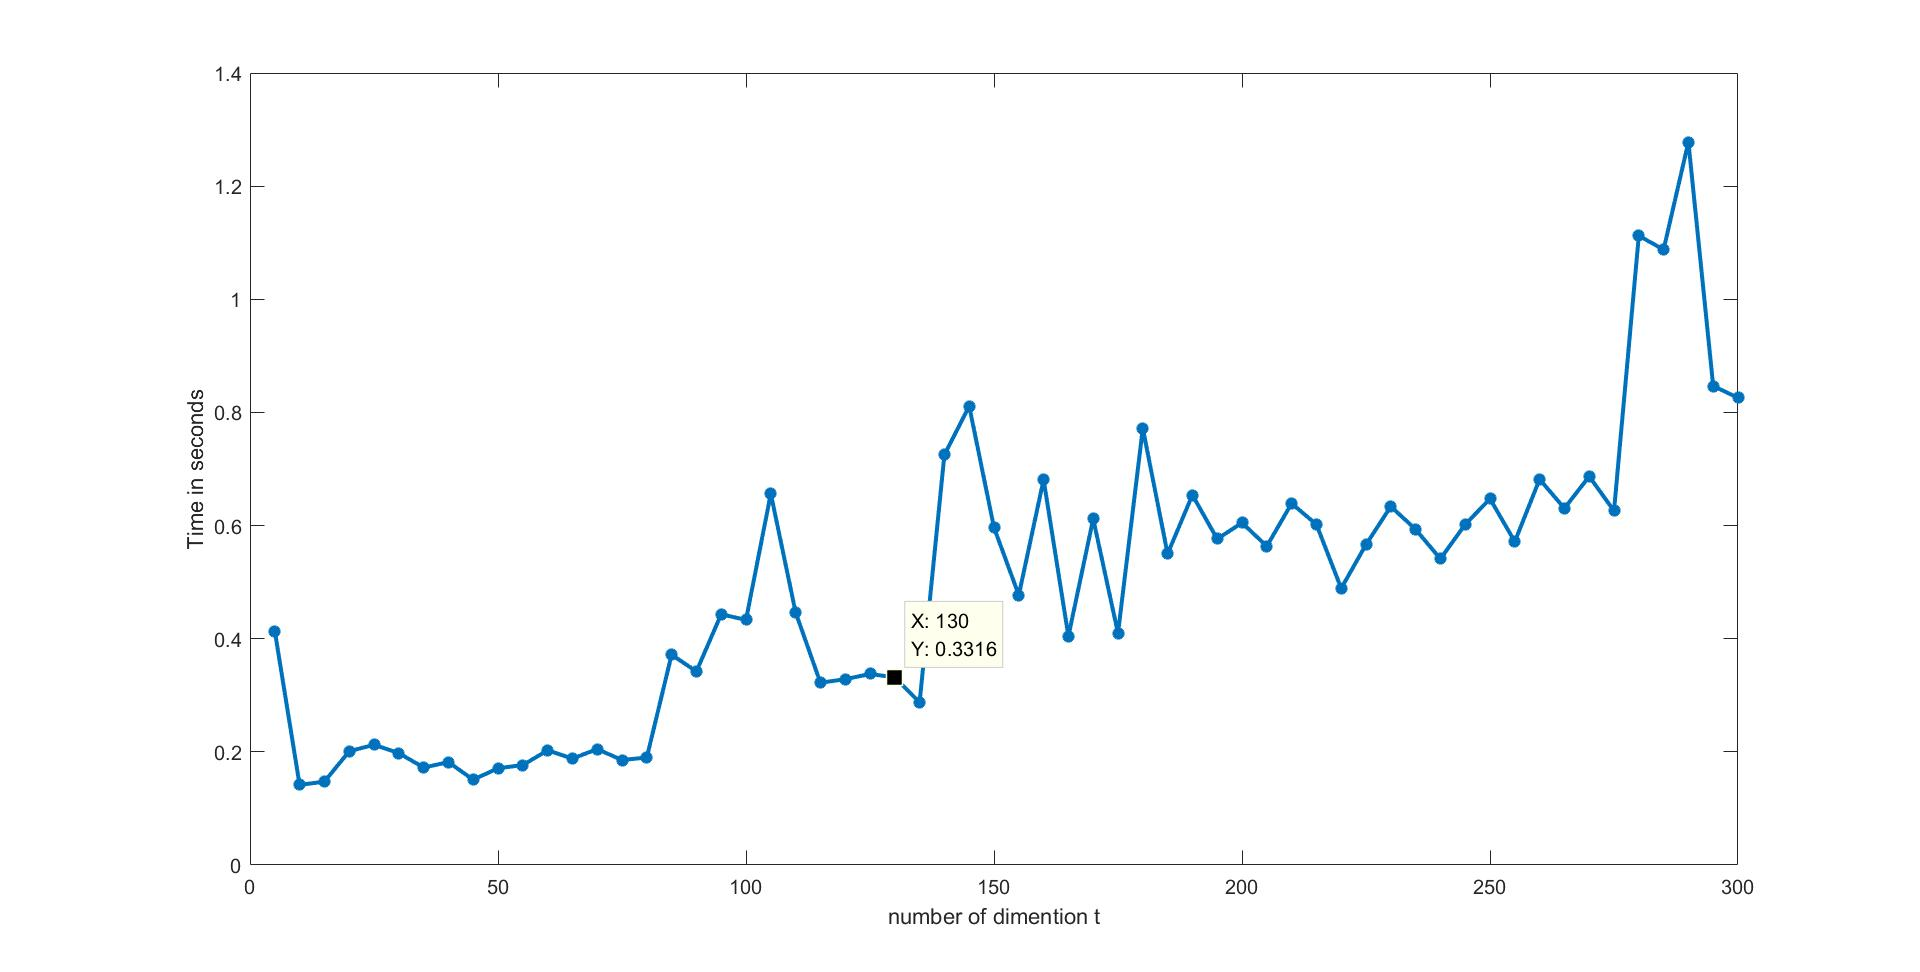
\includegraphics[width=0.50\textwidth]{time.jpg}
        \caption{算法运行的总时间}
        \label{3}
        \end{figure}

    可以看出随着t的增长除了执行时间一直在增长之外,目标函数和准确率的变化趋势逐渐减小,从这次实验的结果看大概在维度是130的时候,目标函数和准确率可以达到几乎最优的程度,再继续增加t结果变化程度比较小,同时在这个维度执行时间也比较短。

    \subsection{思考与改进}
    因为这种基于随机投影的降维方法可解释性不是特别强,我们暂时没有想到怎样从精度上做改进,下面的改进思路主要都是在速度上的\\
    主要的三个改进思路分别是
    \begin{enumerate}
    \item 构造新的随机投影矩阵
    \item 使用mailman算法加速矩阵向量乘法
    \item 多次实验取最好的结果
    \end{enumerate}

    \subsubsection{构造新的随机投影矩阵}
    下面除了论文中随机投影矩阵的构造方法之外,另外使用三种随机投影矩阵的构造方法
    \begin{itemize}
    \item $\forall i,j \quad R_{i,j} \sim N(0,1)$
    \item 在本实验随机矩阵的基础上,使用稀疏矩阵,满足
    \begin{equation*}
    R_{ij} = \begin{cases} +\sqrt{3}/\sqrt{t},& \mbox{w.p. 1/6,} \\0, & \mbox{w.p. 2/3,} \\ -\sqrt{3}/\sqrt{t}, & \mbox{w.p. 1/6.}\end{cases}
    \end{equation*}
    \item Fast JL变换\\
    构造$\Phi = PHD$,其中$P \in R^{k \times d}, H,D \in R^{d \times d}$\\
    P的构造如下:
    \begin{equation*}
    P_{ij} = \begin{cases} N(0,1/q),& \mbox{w.p. q,} \\0, & \mbox{w.p. 1-q}\end{cases}\\
    q = min\Bigl\{ \theta \Bigl(\frac{log^2 n}{d}\Bigr),1 \Bigr\}
    \end{equation*}
    在本实验中q的取值大约为0.07左右,可以看出P非常稀疏,H是归一化的Hadamard矩阵,D是对角矩阵,对角线元素以1/2概率取-1或1.\\
    理论上FJLT的方法可以达到$\theta(nd/\varepsilon^2)$的时间复杂度,这里要求d是二的幂次,所以使用了64*64的ORL数据集
    \end{itemize}

    首先比较一下算法各个部分所用的时间,结果如\ref{time4}.
    \begin{figure}[h]
        \centering
        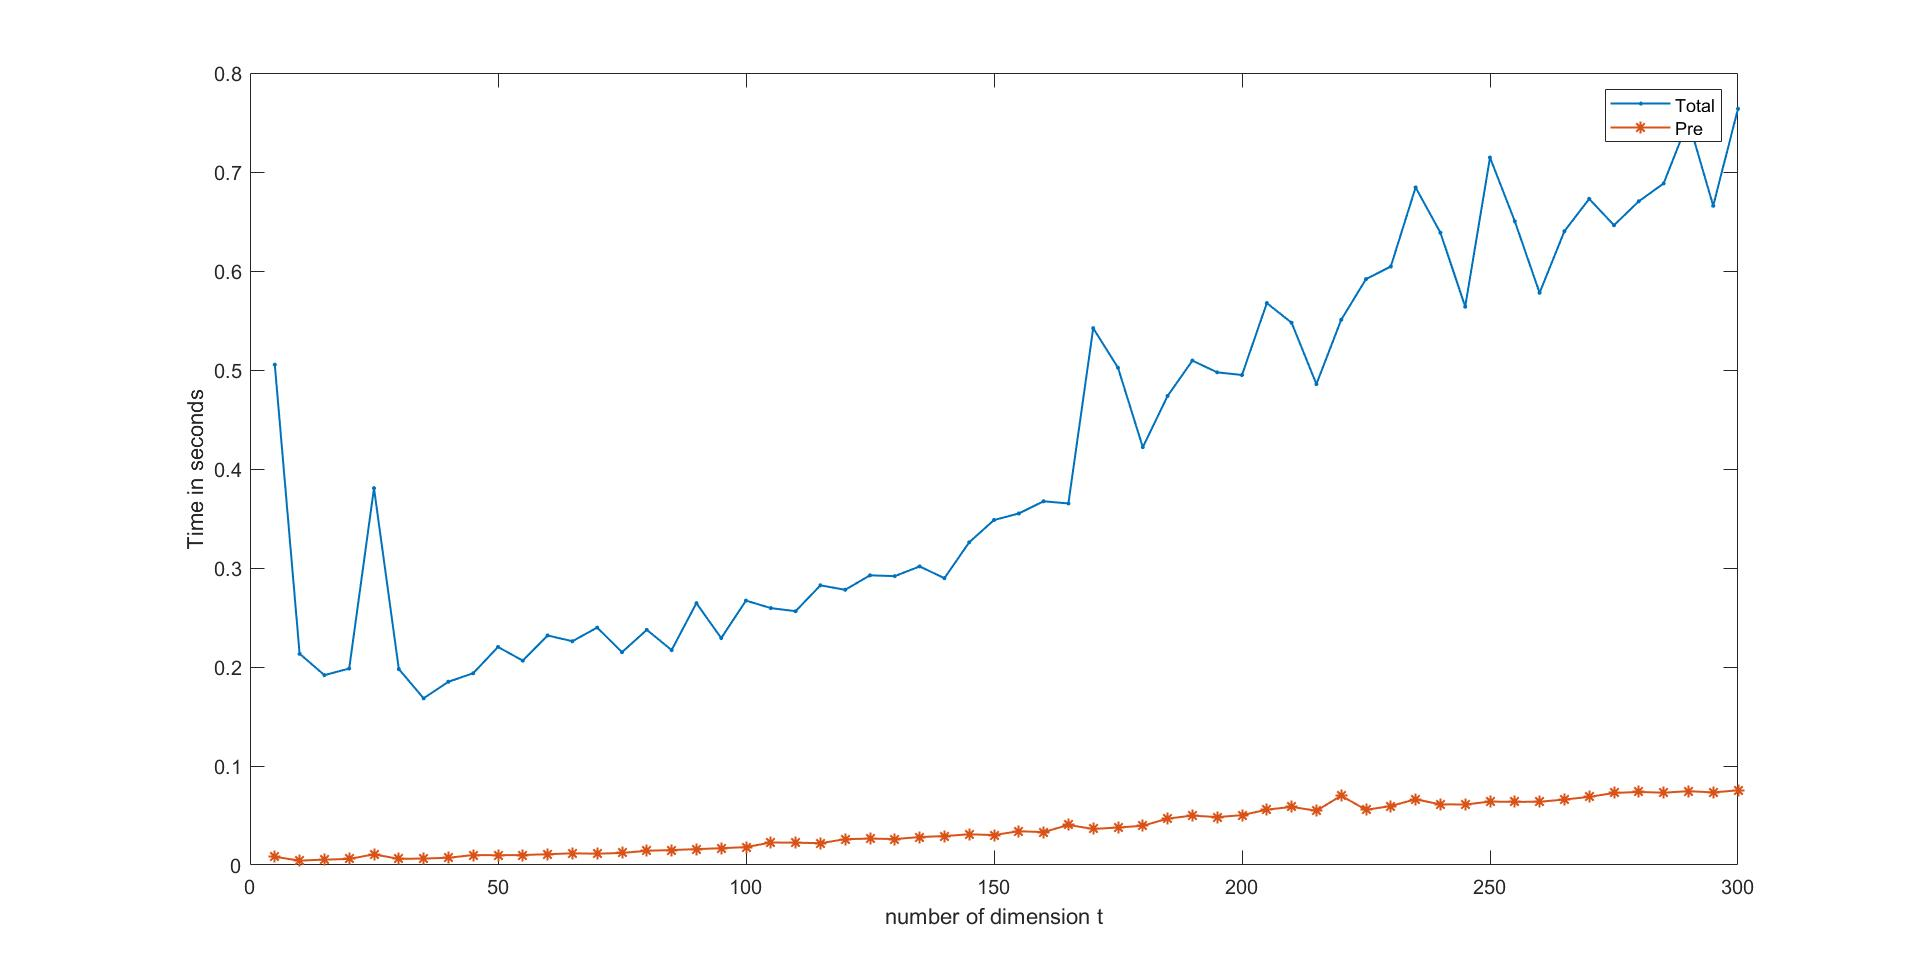
\includegraphics[width=0.50\textwidth]{total_pre.jpg}
        \caption{算法总时间和预处理时间}
        \label{time4}
    \end{figure}

    这里把除了k-means算法之外的计算时间称为预处理时间,可以看到k-means算法的时间是整个算法主要的时间开销,所以不再单独比较四种JL变换的预处理时间\\

    比较四种随机投影矩阵的分类准确率,结果如\ref{accu4}.
    \begin{figure}[h]
        \centering
        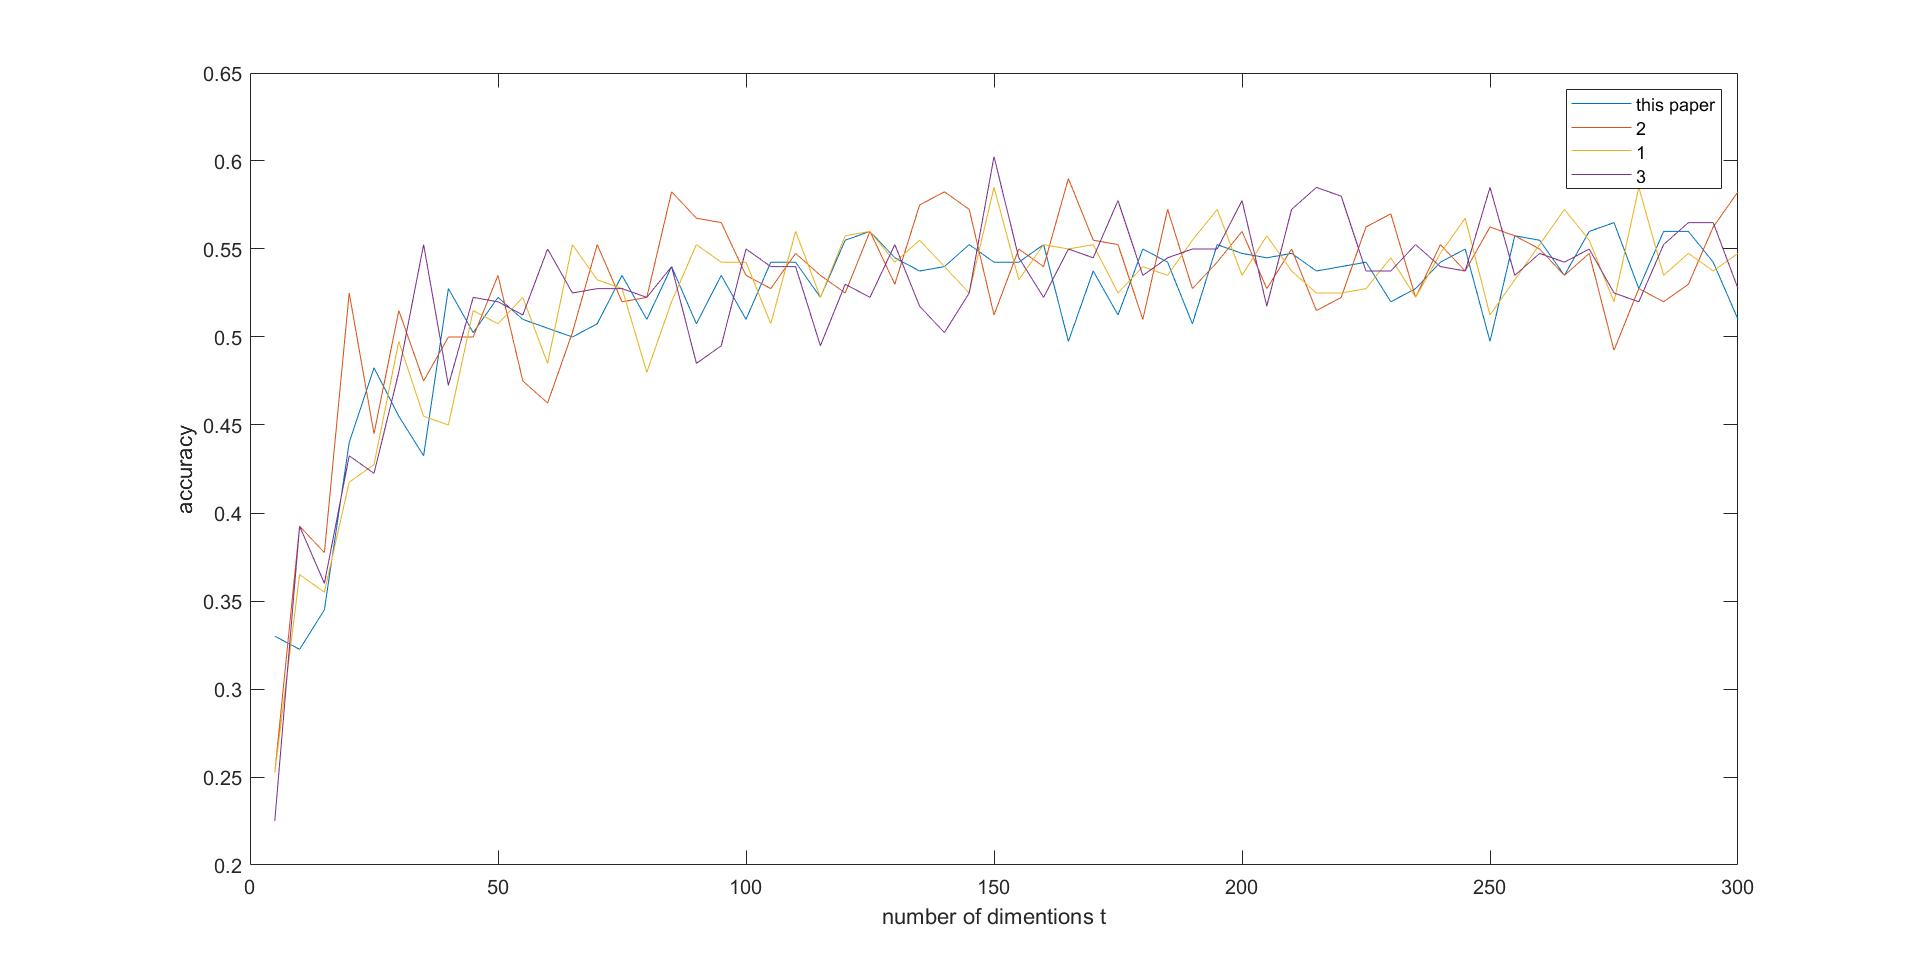
\includegraphics[width=0.50\textwidth]{accu.jpg}
        \caption{四种随机投影矩阵的分类准确率比较}
        \label{accu4}
    \end{figure}

    考虑随机性等原因,我们认为使用这四种随机投影矩阵进行降维并用在k-means中对于分类准确率影响不大.\\

    \subsubsection{使用mailman算法加速矩阵向量乘法}
    当矩阵A的每个元素只取固定的值时,mailman算法能够把矩阵向量乘法$A\vec{x}$的时间复杂度从$O(mn)$降到$O(mn/log(max{m,n}))$
    Mailman算法的核心思想是矩阵向量乘法$A\vec{x}$,其中$A \in R^{m \times n}, \vec{x}\in R^{n \times 1}$可以分解成以下形式\\
    \begin{equation*}
    A\vec{x} = \sum_{i=1}^n A^{(i)}x^{(i)}
    \end{equation*}
    其中,$A^{(i)}$表示A的第i列,$x^{(i)}$表示x的第i个元素,如果想象成是邮递员在送信,$A^{(i)}$就是地址,$x^{(i)}$是信,整个矩阵向量乘法就是邮递员遍历不同的地址送不同的信,但是因为地址是确定的,原始的乘法只是机械地走完全程,并没有考虑地址相同的情况。\\

    下面简单描述一下如何使用mailman算法计算矩阵向量乘法,这里不妨假设$ m = log_2^n$,并且$A(i,j) \in {0,1}$,如果不是可以把矩阵分成子矩阵或再进行扩展.
    构造两个新矩阵$U_{n}$和$n \times n$的矩阵P,$U_{n}$的每一列存储可能出现的由m个{0,1}组成的向量,那么A的每一列在$U_{n}$中都会出现。$P(i,j) = \delta(U^{(i)},A^{(j)})\quad \delta = 1 \quad \text{if} \quad U^{(i)} = A^{(j)}$,所以P只有n个非零元。
    \begin{align*}
    \because (U_{n}P)(i,j) &=\sum_{k=1}^n U_{n}(i,k)P(k,j)\\
    &=\sum_{k=1}^n U_{n}^{(k)}(i)\delta (U_{n}^{(k)},A^{(j)})\\
    &=A(i,j)\\
    \therefore A\vec{x} &=(UP)\vec{x} = U(P\vec{x})\\
    \end{align*}
    因为P只有n个非零元,计算$P\vec{x}$的时间复杂度为$O(n)$,利用二的幂次的性质,递归计算$U(P\vec{x})$的时间复杂度也为$O(n)$,更一般的情况下,在使用随机投影降维的算法中,理论上时间复杂度可以降低$max\{n,d\}$,但是不论是在mailman算法的原始文献中还是在随机投影降维的文章中,作者都表示实际无法达到理论效果,所以并没有对该算法进一步尝试。

    \addcontentsline{toc}{section}{参考文献}
    \nocite{*} % So we don't need to explicitly cite them
    \bibliographystyle{plain}
    \bibliography{ref}
\end{document}
